% Documentation note — the PTCryspMC scanner productions: the two representative systems,
% the CTR findings/calibration, the source activity + positioning, and the deliverables for
% CryspBrainSim. Compiles with pdflatex; figures live in latex/figures/ (embedded in the built
% PDF, so the published PDF is self-contained). No .bib.
% A copy of the built PDF is published at the PtCryspProds root by publish_prod.jl.
\documentclass[11pt,a4paper]{article}

\usepackage[margin=2.6cm]{geometry}
\usepackage{amsmath}
\usepackage{booktabs}
\usepackage{graphicx}
\usepackage[colorlinks=true, linkcolor=blue!50!black, citecolor=blue!50!black, urlcolor=blue!50!black]{hyperref}
\usepackage{xcolor}

\newcommand{\Ndet}{N_{\mathrm{det}}}
\newcommand{\ns}{\,\mathrm{ns}}
\newcommand{\ps}{\,\mathrm{ps}}
\newcommand{\keV}{\,\mathrm{keV}}

\title{The \textsc{PTCryspMC} scanner productions:\\
       the two representative systems, the timing calibration (CTR),\\
       and the deliverables for \textsc{CryspBrainSim}}
\author{PTCryspMC.jl documentation note}
\date{July 2026}

\begin{document}
\maketitle

\begin{abstract}
\noindent
The first version of the \textsc{PTCryspMC} timing model stamped each detected gamma with the
arrival time of its \emph{first} scintillation photon. That model is internally consistent but
represents only the photostatistics floor: for cryogenic CsI it predicts a coincidence time
resolution (CTR) of $49\ps$ FWHM, a factor ${\sim}40$ better than the measured $1.84\ns$
\cite{Soleti2024}. This note documents the finding, decomposes the discrepancy
(photon statistics vs.\ optical transport vs.\ trigger electronics), and describes the adopted
solution: a per-crystal Gaussian \emph{readout floor} $\sigma_t$, added to the physical
first-photon term and calibrated to bench measurements and to the operating point of commercial
BGO systems. With the calibrated model, the simulated raw time-difference widths are
$\sigma \simeq 0.51\ns$ (CsI) and $1.77\ns$ (BGO at 77\,K and at 195\,K, indistinguishable),
and the pinned coincidence windows $\tau = 1.5\ns$ (CsI) and $5\ns$ (BGO) sit at
${\sim}3\sigma$, keeping $99.7\%$ and $99.3\%$ of true coincidences respectively.
The note closes with the production deliverables (section~\ref{sec:deliverables}): a
scanner-geometry survey --- eight ring designs (radius $200$--$387$\,mm, AFOV $30$--$102$\,cm),
each in both crystals, from the identical proton-activity source, five promoted to ten-shard
masters --- with the geometry, statistics, file layout and column semantics the downstream
\textsc{CryspBrainSim} analysis consumes.
\end{abstract}

\section{Context and definitions}

\textsc{PTCryspMC} is a fast, photon-only Monte Carlo of a PET ring: it transports the two
$511\keV$ annihilation gammas, forms per-crystal hits, and writes the list-mode coincidence
(LOR) file. Scintillation light is \emph{not} tracked photon by photon; the timing of each
detected gamma is produced by an analytic model evaluated once per hit. Three crystal systems
are simulated (table~\ref{tab:systems}): pure CsI at ${\sim}100$\,K, and BGO at two cryogenic
operating points, 195\,K (dry ice) and 77\,K (liquid nitrogen). All three share the same ring
(transverse block size, $48\times20$ blocks) with a per-crystal depth of \textbf{two radiation
lengths} --- the standard adopted because the CRYSP position/DOI resolution of
$3.5$\,mm FWHM per axis is measured on $2X_0$ crystals with the SiPM readout (deeper crystals
would degrade the light-based position estimate and raise cost; a $3X_0$ variant is kept in
the repository for a future thick-crystal study).

Two time-difference quantities must be kept distinct:
\begin{itemize}
\item $\Delta t_{\mathrm{raw}} = t_1 - t_2$, the \textbf{window variable}: the difference of the
  two measured arrival times. It physically contains the time-of-flight (TOF) difference of the
  two gammas --- including each gamma's depth-of-interaction (DOI) penetration --- convolved
  with the detector timing response. A scanner cuts on
  $|\Delta t_{\mathrm{raw}}| \le \tau$; nothing is, or can be, corrected for TOF, since the
  emission point is unknown in a measurement.
\item $dt = (t_1 - t_2) - \Delta\mathrm{TOF}$, the \textbf{TOF-corrected residual}: the
  detector-only response, computable in the simulation because the true emission point is
  known. It is what a bench measurement with a centred point source calls CTR (there the two
  TOFs are equal and cancel). In the simulation output it is a truth-level diagnostic; it is
  never used in any selection.
\end{itemize}

\begin{table}[ht]
\centering
\caption{The three simulated crystal systems. Light yield $Y$, decay components
$\tau_k$ with weights $w_k$, energy resolution $a$ (FWHM at $511\keV$), effective photon
detection efficiency (PDE), depth (2\,$X_0$), position/DOI resolution, photopeak selection
($E_{\mathrm{min}} = 511 - 3\sigma_E$), and the calibrated readout floor $\sigma_t$
(section~\ref{sec:model}). CsI constants follow the measurements of ref.~\cite{Soleti2024}
($\,{\sim}90{,}000$ photons/MeV, single ${\sim}800\ns$ component at 104\,K, $6.3\%$ FWHM);
BGO cryogenic constants from the CRYSP programme. The PDE corresponds to the Hamamatsu
S14160-6050HS ($\sim$40\% at the CsI 350\,nm cryogenic emission; the BGO band sits at longer
wavelengths where the sensor response is similar or better), with light-collection efficiency
taken as ${\approx}1$ for the large monolithic blocks pending a dedicated optical MC.}
\label{tab:systems}
\vspace{2mm}
\begin{tabular}{lccc}
\toprule
 & CsI (${\sim}100$\,K) & BGO (195\,K) & BGO (77\,K) \\
\midrule
$Y$ (photons/MeV)            & $100{,}000$   & $14{,}000$ & $29{,}000$ \\
$\tau_k$ (ns)                & 800           & 1768       & 1400 / 8700 \\
$w_k$                        & 1.0           & 1.0        & 0.26 / 0.74 \\
$a$ (FWHM at 511 keV)        & 6\%           & 15\%       & 10\% \\
PDE                          & 0.40          & 0.40       & 0.40 \\
depth $= 2X_0$ (cm)          & 3.720         & 2.236      & 2.236 \\
$\sigma_{xyz}$ (FWHM, per axis) & 3.5\,mm    & 3.5\,mm    & 3.5\,mm \\
$E_{\mathrm{min}}$ (keV)     & 472           & 413        & 446 \\
$\sigma_t$ (ns)              & 0.35          & 1.1        & 1.1 \\
coincidence window $\tau$ (ns) & 1.5         & 5.0        & 5.0 \\
\bottomrule
\end{tabular}
\end{table}

\section{The first-photon model and why it is a floor}
\label{sec:firstphoton}

A deposit of energy $E$ is assumed to produce
\begin{equation}
  \Ndet = Y \, E \, \mathrm{PDE}
\end{equation}
detected scintillation photons. Each photon's emission time follows the decay mixture
$f(t) = \sum_k (w_k/\tau_k)\, e^{-t/\tau_k}$, whose rate at early times is
$r_0 = f(0) = \sum_k w_k/\tau_k$. Since the first arrival occurs at times far below the decay
constants, the minimum of $\Ndet$ such draws is exponential with rate $\Ndet\, r_0$:
\begin{equation}
  t_{\mathrm{jitter}} = -\frac{\ln u}{\Ndet\, r_0}, \qquad u \sim \mathcal{U}(0,1),
  \qquad \langle t_{\mathrm{jitter}} \rangle = \frac{1}{\Ndet\, r_0}.
  \label{eq:firstphoton}
\end{equation}
For a full-energy $511\keV$ deposit this gives a mean jitter of $39\ps$ per gamma for CsI
($\Ndet \approx 20{,}400$) and ${\approx}0.62\ns$ for both BGO systems
($\Ndet \approx 5{,}900$ at 77\,K, $2{,}900$ at 195\,K --- the lower yield at 195\,K is almost
exactly compensated by its faster decay, a degeneracy that persists throughout this note).
The difference of two independent exponentials is Laplace-distributed, so the model predicted
CTR values of $49\ps$ (CsI) and ${\approx}0.78\ns$ (BGO) FWHM.

Two properties of eq.~\eqref{eq:firstphoton} are worth keeping: the correct scaling of the
photostatistics term with deposited energy (a low-energy crystal deposit has few photons and
poor timing --- the time spread grows as $1/E$), and its correct dependence on yield, PDE and
decay mixture. What it omits is everything downstream of photon emission.

\section{Confrontation with measurement}
\label{sec:measurement}

Soleti et al.~\cite{Soleti2024} measured pure CsI at 104\,K
($3\times3\times20$\,mm$^3$ crystals, PTFE-wrapped, one $3\times3$\,mm$^2$ MPPC each):
light yield ${\sim}90{,}000$ photons/MeV, a single ${\sim}800\ns$ decay component, energy
resolution $6.3\%$ FWHM --- all in agreement with the constants of table~\ref{tab:systems} ---
and a \textbf{CTR of $1.84 \pm 0.07\ns$ FWHM}, using leading-edge time pick-off at five times
the electronic noise, in a photopeak energy window.

The bench photoelectron count was $N_{\mathrm{pe}} \approx 4{,}600$ (PDE 17\% for that MPPC at
the cryogenic emission spectrum, light-collection efficiency 58\% for the narrow crystal
geometry). Even at that $N_{\mathrm{pe}}$, the ideal first-photon bound of
eq.~\eqref{eq:firstphoton} is ${\sim}0.24\ns$ FWHM --- a factor $7$--$8$ below the measurement.
The remainder is the readout: a fixed-voltage leading-edge threshold on a pulse that rises with
an $800\ns$ decay constant crosses at an effective depth of order ten photoelectrons, with
residual time walk on top. Tellingly, the authors observed that \emph{lowering} the threshold
below $3\sigma$ of the noise \emph{worsened} the CTR: the noise floor forbids true first-photon
timing. The measured CTR is therefore \textbf{electronics/trigger dominated}, and the
first-photon term of section~\ref{sec:firstphoton} is a small correction to it.

The intermediate contribution --- optical transport inside the crystal --- is small for the
geometries simulated here. The bench's 58\% collection efficiency was the price of a $20{:}7$
aspect-ratio needle with many wall reflections; the scanner's large monolithic blocks with
full-face readout reflect far less (PTFE reflectivity is ${\sim}95\%$ \cite{Janecek2012}), and
the DOI-dependent light-transit spread across the block depth amounts to
$\sigma \approx 40$--$60\ps$ per gamma. The hierarchy of per-gamma contributions is then:

\begin{center}
\begin{tabular}{lcc}
\toprule
per-gamma term & CsI & BGO (both) \\
\midrule
photostatistics floor (modelled, eq.~\ref{eq:firstphoton}) & $39\ps$  & $620\ps$ \\
optical transit (unmodelled)                               & ${\sim}50\ps$ & ${\sim}50\ps$ \\
electronics / trigger (unmodelled)                         & \textbf{dominant} & subdominant \\
\bottomrule
\end{tabular}
\end{center}

For BGO no equivalent cryogenic bench CTR exists yet. Extrapolating from the CsI anchor with
the standard scintillator figure of merit $\mathrm{CTR} \propto \sqrt{\tau/N_{\mathrm{ph}}}$
\cite{Conti2009} (the scaling law also used by ref.~\cite{Soleti2024} for its own
extrapolations), both BGO operating points land at ${\approx}4\times$ the CsI CTR. This is
consistent with the ${\sim}5\ns$ coincidence window at which commercial whole-body BGO systems
operate, e.g.\ the GE Omni Legend~32 \cite{Yamagishi2023}, which we take as the realistic
operating point.

\section{How the model handles it}
\label{sec:model}

The adopted timestamp of a detected gamma is
\begin{equation}
  t \;=\; \mathrm{TOF}(\text{annihilation} \to \text{first interaction})
     \;+\; t_{\mathrm{jitter}}
     \;+\; \sigma_t \cdot g, \qquad g \sim \mathcal{N}(0,1),
  \label{eq:stamp}
\end{equation}
where $t_{\mathrm{jitter}}$ is the physical first-photon draw of eq.~\eqref{eq:firstphoton}
and $\sigma_t$ is a per-crystal Gaussian \textbf{readout floor} lumping the trigger/threshold
statistics, the SiPM single-photon transit spread, and the optical transit --- everything a
leading-edge readout adds on top of photon emission. The physical term is kept because it is
free, carries the correct $1/E$ deterioration for low-energy deposits, and is genuinely the
dominant term for slow low-yield crystals; the Gaussian term carries the measured reality.
TOF is the gamma's flight to its own first interaction point, so the DOI penetration is
inside each $t$ and hence inside $\Delta t_{\mathrm{raw}}$ --- consistent with a measurement,
where DOI is likewise absorbed into the arrival times. No TOF correction is applied anywhere
in the selection chain.

The calibration of $\sigma_t$:
\begin{itemize}
\item \textbf{CsI: $\sigma_t = 0.35\ns$.} Anchored to the measured $1.84\ns$ FWHM
  \cite{Soleti2024} at $N_{\mathrm{pe}} = 4{,}600$, scaled by
  $\sqrt{N}$ to the scanner assumption $\Ndet \approx 20{,}400$
  (PDE 0.40 with the Hamamatsu S14160-6050HS and near-unity collection in the large block),
  and chosen so that the total raw width satisfies $3\sigma \approx 1.5\ns$, the pinned window.
\item \textbf{BGO (both): $\sigma_t = 1.1\ns$.} From the $\mathrm{CTR} \propto
  \sqrt{\tau/N_{\mathrm{ph}}}$ extrapolation of the CsI anchor \cite{Conti2009}, and chosen so
  that $3\sigma \approx 5\ns$, matching the window of the commercial BGO reference
  \cite{Yamagishi2023}. To be replaced by a direct calibration when a cryogenic BGO bench CTR
  becomes available.
\end{itemize}

One methodological point: the CTR study must be conditioned on the photopeak energy selection
($E \ge 511 - 3\sigma_E$ per crystal, table~\ref{tab:systems}). The uncut coincidence list
contains few-keV crystal deposits whose photostatistics jitter, by the $1/E$ scaling of
eq.~\eqref{eq:firstphoton}, reaches $10^2$--$10^5\ns$; these events dominate a naive standard
deviation but never survive the energy selection that precedes any timing cut in the real
chain.

\section{Validated results and the coincidence windows}
\label{sec:results}

The model was validated with one full production shard per scanner ($8\times10^7$ decays of a
1\,Gy proton-therapy activity scenario in a head phantom; $6$--$15$~million
energy-selected true coincidences each), run at the production $2X_0$ geometry.
Table~\ref{tab:results} shows the measured widths and the containment at the pinned windows.
(The study was first run at $3X_0$ and repeated at $2X_0$: the widths agree within $0.3\%$ ---
the DOI contribution to $\Delta t_{\mathrm{raw}}$ is negligible against the readout floor.)

\begin{table}[ht]
\centering
\caption{Simulated timing with the calibrated model (one shard per scanner at the production
$2X_0$ geometry, photopeak-selected). $\sigma_{\mathrm{raw}}$ is the width of the window
variable $\Delta t_{\mathrm{raw}}$ (it includes the TOF spread of the source across the head
phantom and the DOI spread); the CTR column is the FWHM of the TOF-corrected residual (the
bench-equivalent detector response). The pinned windows sit at ${\sim}3\sigma$. BGO 77\,K
(not scheduled for production) is timing-identical to 195\,K to three digits.}
\label{tab:results}
\vspace{2mm}
\begin{tabular}{lccccc}
\toprule
scanner & $\sigma_{\mathrm{raw}}$ & CTR (FWHM) & $\tau$ & $\tau/\sigma_{\mathrm{raw}}$ &
trues kept at $\tau$ \\
\midrule
CsI       & $0.510\ns$ & $1.16\ns$ & $1.5\ns$ & $2.9$ & $99.67\%$ \\
BGO 195\,K & $1.77\ns$  & $4.10\ns$ & $5.0\ns$ & $2.8$ & $99.31\%$ \\
\bottomrule
\end{tabular}
\end{table}

Findings:
\begin{enumerate}
\item \textbf{The calibrated CsI CTR is $1.17\ns$ FWHM} --- consistent with the bench
  measurement of ref.~\cite{Soleti2024} once the improved sensor (PDE $0.17 \to 0.40$) and the
  block light collection are credited, and a factor ${\sim}24$ more conservative than the
  original first-photon prediction.
\item \textbf{The two BGO operating points are indistinguishable in timing} (widths equal to
  three digits): the 195\,K yield loss is compensated by its faster decay at every level of the
  modelling --- first-photon mean, figure-of-merit extrapolation, and full MC. The choice
  between them is therefore purely an energy-resolution choice ($10\%$ vs.\ $15\%$ FWHM),
  i.e.\ scatter rejection, not timing.
\item \textbf{The pinned windows behave as $3\sigma$ Gaussian cuts.} With the Gaussian floor
  dominant, the raw $\Delta t$ distributions are Gaussian to good accuracy (robust and standard
  widths agree to $0.1\%$), and the earlier concern about heavy Laplace tails --- which made
  $3\sigma$ keep only $97\%$ when the exponential term dominated --- has dissolved.
\item \textbf{For CsI the window is not detector-limited.} Its raw width
  ($0.51\ns$) is dominated by the readout floor and the TOF/DOI geometric spread in comparable
  parts; the photostatistics term ($39\ps$) is negligible. Any further sensor improvement
  changes CsI's window only marginally --- the head geometry is already visible in it.
\end{enumerate}

\section{The two representative scanners}
\label{sec:twoscanners}

The first production campaign simulates two of the three systems: \textbf{BGO at 195\,K} and
\textbf{cryogenic CsI}. The choice follows directly from the findings above:

\begin{itemize}
\item \textbf{BGO 77\,K adds no timing information over 195\,K.} The two BGO operating points
  are timing-degenerate at every level of modelling (section~\ref{sec:results}); they differ
  only in energy resolution ($10\%$ vs.\ $15\%$) and cryogenic cost (liquid nitrogen vs.\ dry
  ice, plus a ${\sim}4\times$ longer integration window at 77\,K from the $8.7\,\mu$s slow
  component). BGO 195\,K is therefore the representative BGO: the cheaper operating point,
  with the 77\,K configuration kept ready should the energy-resolution margin matter.
\item \textbf{CsI vs.\ BGO 195\,K spans the physics contrast cleanly.} CsI buys energy
  resolution ($6\%$ vs.\ $15\%$ FWHM $\to$ a photopeak cut at $472$ vs.\ $413\keV$, i.e.\
  stronger scatter rejection) and timing ($\tau = 1.5$ vs.\ $5\ns$ $\to$ ${\sim}3\times$ fewer
  randoms at equal rate); BGO buys sensitivity ($87\%$ vs.\ $78\%$ per-gamma interaction
  probability at $2X_0$, i.e.\ ${\sim}24\%$ more coincidences at equal source) at a lower
  cryogenic operating cost. Position resolution and ring geometry are identical by
  construction, so the downstream range-precision comparison isolates exactly these two axes.
\end{itemize}

Per-SiPM light levels support both choices: with an $8\times8$ SiPM array per block, the mean
photopeak signal is ${\sim}45$ photoelectrons per SiPM for BGO 195\,K and ${\sim}320$ for CsI.
With dark counts frozen out at cryogenic temperatures (the rate halves every ${\sim}5$\,K
\cite{Soleti2024}), ${\sim}45$\,pe per SiPM is comfortable statistics; BGO's larger
photoelectric fraction at $511\keV$ (high-$Z$ bismuth) additionally yields cleaner single-site
deposits for the light-based position estimator.

\section{Production deliverables for \textsc{CryspBrainSim}}
\label{sec:deliverables}

The productions form a \textbf{scanner-geometry survey}: the same block module, crystal
systems, detector constants and identical proton-activity source, over a family of closed rings
that vary only in \emph{radius} and \emph{axial length}. The aim is the range-precision figure
$\sigma_R$ as a function of geometry, at fixed physics. Files land in the \texttt{PtCryspProds/}
tree (layout contract: \texttt{PRODUCTS.md} = the tree's \texttt{README.md}; column schema:
\texttt{SCHEMA.md} at the tree root, refreshed on every publish, as is this note's PDF).

Each leaf, at \texttt{<scanner>/<crystal>/fast\_1Gy/} under the scenario, holds
\texttt{lors\_shardNNN.h5} plus \texttt{config.toml} (the regeneration recipe);
\texttt{scanner\_geometry.json} sits at the scanner level, and the shared \texttt{phantom/}
($\mu$-map inputs) and \texttt{truth/} (dose-$R_{80}$ + activity-$R_{50}$) bundles at the
scenario level. Every arm exists in \textbf{both} crystals (BGO 195\,K and CsI). A leaf carries
\textbf{ten shards} (a full master, $\Sigma M \approx 8.0\times10^8$ decays) or \textbf{one
shard} (a survey point sufficient for acceptance / composition, promotable to a master on
request):

\begin{center}
\small\setlength{\tabcolsep}{5pt}
\begin{tabular}{lccccc}
\toprule
scanner & radius & AFOV & $\varphi\times z$ blocks & crystal area & shards \\
\midrule
\texttt{crysp\_ring\_1m}   & 387\,mm & 1024\,mm & $48\times20$ & 2.49\,m$^2$ & \textbf{10} \\
\texttt{crysp\_r35\_50cm}  & 350\,mm & 512\,mm  & $43\times10$ & 1.13\,m$^2$ & \textbf{10} \\
\texttt{crysp\_r35\_35cm}  & 350\,mm & 358\,mm  & $43\times7$  & 0.79\,m$^2$ & \textbf{10} \\
\texttt{crysp\_r30\_30cm}  & 300\,mm & 307\,mm  & $37\times6$  & 0.58\,m$^2$ & \textbf{10} \\
\texttt{crysp\_chs}        & 200\,mm & 358\,mm  & $25\times7$  & 0.45\,m$^2$ & \textbf{10} \\
\texttt{crysp\_r30\_50cm}  & 300\,mm & 512\,mm  & $37\times10$ & 0.97\,m$^2$ & 1 \\
\texttt{crysp\_ring\_50cm} & 387\,mm & 512\,mm  & $48\times10$ & 1.25\,m$^2$ & 1 \\
\texttt{crysp\_r35\_30cm}  & 350\,mm & 307\,mm  & $43\times6$  & 0.68\,m$^2$ & 1 \\
\bottomrule
\end{tabular}
\end{center}

Scanner names append the crystal and depth ($\ldots$\texttt{\_bgo\_2x0}, $\ldots$\texttt{\_csi\_2x0});
the CHS is the \emph{compact head scanner} (200\,mm crystal radius $\to$ ${\sim}30$\,cm patient
bore after the cryostat, the ring sliding over the head with its lower edge at the shoulder
line, vertex-to-C7).

\subsection*{Scanner geometry}

Every scanner is a closed cylindrical ring built from the \textbf{same monolithic block}: a
transverse face of $50.6$\,mm (arc at the inner radius) $\times\, 51.2$\,mm ($z$ wheel pitch),
at $2X_0$ depth --- $22.36$\,mm for BGO (outer radius $=$ inner $+\,22.36$\,mm) and $37.20$\,mm
for CsI (inner $+\,37.20$\,mm). The block face is fixed, so the $\varphi\times z$ block counts of
the survey table quantize the chosen radius and AFOV. The detector response
(table~\ref{tab:systems}) --- $\sigma_{xyz}$, energy resolution, photopeak cut, $\tau$ --- is
identical across all rings and already applied in the files; do \emph{not} re-apply it.

The phantom is the scenario's, identical for every arm: a uniform G4\_BRAIN\_ICRP ellipsoid
(semi-axes $7.2 \times 8.7 \times 10.2$\,cm, centred at $(0, -3, 0)$\,cm), inside an air world.
It is contained even by the shortest ring (its $\pm 102$\,mm axial extent inside the
$\pm 154$\,mm FOV of the 30\,cm arms), so the SOBP distal edge --- near the axial centre --- sits
where every ring is efficient.

\subsection*{Source and statistics}

The source is the frozen \texttt{uniform\_headep\_sobp\_1e8} scenario at 1\,Gy over the
acquisition window $[0, 1200]$\,s: ${\approx}8.02\times10^7$ decays per shard,
5 isotopes ($^{15}$O, $^{11}$C, $^{13}$N, $^{10}$C, $^{14}$O). Shard $R$ is seeded by
(\texttt{master\_seed}=1, \texttt{realization}=$R$), and \textbf{the same $R$ sees the identical
annihilation set on \emph{every} scanner and crystal} --- all differences across the survey are
detector/geometry-only, event by event.

Measured shard-0 statistics across the survey (detector-level acceptance = fraction of the
$8.0\times10^7$ annihilations surviving containment, photopeak cut and the DT window):

\begin{center}
\begin{tabular}{lcccc}
\toprule
scanner & \multicolumn{2}{c}{acceptance} & \multicolumn{2}{c}{det.\ LORs / shard} \\
        & BGO 195\,K & CsI & BGO 195\,K & CsI \\
\midrule
\texttt{ring\_1m}   (R387$\times$1024) & $19.0\%$ & $7.6\%$  & $15.3$\,M & $6.1$\,M \\
\texttt{r30\_50cm}  (R300$\times$512)  & $13.6\%$ & $5.35\%$ & $10.9$\,M & $4.3$\,M \\
\texttt{chs}        (R200$\times$358)  & $12.7\%$ & $4.9\%$  & $10.1$\,M & $3.9$\,M \\
\texttt{r35\_50cm}  (R350$\times$512)  & $12.1\%$ & $4.78\%$ & $9.7$\,M  & $3.8$\,M \\
\texttt{ring\_50cm} (R387$\times$512)  & $11.1\%$ & $4.4\%$  & $8.9$\,M  & $3.5$\,M \\
\texttt{r35\_35cm}  (R350$\times$358)  & $7.8\%$  & $3.11\%$ & $6.3$\,M  & $2.5$\,M \\
\texttt{r35\_30cm}  (R350$\times$307)  & $6.2\%$  & $2.48\%$ & $5.0$\,M  & $2.0$\,M \\
\texttt{r30\_30cm}  (R300$\times$307)  & $7.2\%$  & $2.85\%$ & $5.8$\,M  & $2.3$\,M \\
\bottomrule
\end{tabular}
\end{center}

Two invariants hold across the whole family. \textbf{Purity is geometry-independent}:
${\sim}72$--$75\%$ true / ${\sim}25$--$27\%$ scatter for BGO and ${\sim}87\%$ true / $13\%$
scatter for CsI everywhere, randoms $<0.3\%$ --- so geometry moves only the statistics, and the
CsI-vs-BGO contrast (CsI purer, BGO ${\sim}2.5\times$ the counts) is the crystal axis at every
ring. \textbf{Radius beats length}: at fixed $358$\,mm AFOV, shrinking the crystal radius
$350\to200$\,mm (\texttt{r35\_35cm}$\to$\texttt{chs}) raises BGO acceptance $7.8\to12.7\%$ while
\emph{halving} the crystal area --- solid angle is bought far more cheaply with radius than with
axial length, and the compact head scanner outperforms every $R\ge300$\,mm ring of any length
below $1$\,m. The axial scan is smoother than the raw acceptance suggests for range work: the
source fills two-thirds of the shortest FOV, so the $50\to30$\,cm acceptance loss (${\sim}\times
0.5$) is concentrated at the phantom poles, away from the centrally-located distal edge the
range measurement uses.

Per shard, BGO leaves ${\sim}300$--$490$\,MB and CsI ${\sim}120$--$190$\,MB (scaling with the
LOR count); a ten-shard master pools to $\Sigma M \approx 8.0\times10^8$ decays.

\subsection*{Column semantics (highlights; full schema in \texttt{SCHEMA.md})}

Per LOR: smeared 3-D hit positions and energies of both gammas (quantized Int16, $0.1$\,mm /
$0.1\keV$), the block indices, per-gamma phantom-scatter counts (\texttt{nscat1/2}: 0 clean,
1 single, $\ge 2$ multiple), times $t_1, t_2$ (Float32 ns, \emph{relative to the decay}), the
truth-level timing residual \texttt{dt\_ns}, the true annihilation point
(\texttt{x0/y0/z0\_mm}), the truth flag (0 true / 1 scatter / 2 random), and
\texttt{t\_decay\_s} --- the absolute decay time in the acquisition window, so a delayed
acquisition start is the pure cut $t_{\mathrm{decay}} \ge t_{\mathrm{start}}$ on the stored
list (statistically exact, per-isotope decay laws included; randoms carry gamma~1's decay,
matching the \texttt{x0} convention). Root attributes carry full provenance (scenario, dose,
budget, seeds, detector windows, geometry segmentation).

\subsection*{Relation to the existing reference master}

The pre-existing master at \texttt{crysp\_ring\_1m/bgo/fast\_1Gy/} (ten shards) is
\textbf{frozen}: it predates this standard (hybrid room/cryo BGO constants, $3.7$\,cm depth,
no readout floor, $450\keV$ cut, $\tau = 3\ns$, $\sigma_{xyz} = 1.7$\,mm Gaussian $\sigma$).
It remains valid as a methods reference but must not be pooled or compared quantitatively with
any survey arm.

\section{The v2 convention and the first production round}
\label{sec:activity}

Generation-2 fixes three conventions (full spec: \texttt{generation2\_plan.md}), each recorded in
every shard's HDF5 attributes so a file is self-describing --- guarded by \texttt{generation="v2"}.

\subsection*{Patient placement: tumour-centred}

The patient is placed as in the clinic: the \textbf{tumour} at isocentre --- a fixed anatomical
reference set from NMR/CT \emph{before} any acquisition, not the activity edge (which drifts with the
window). The source and phantom are rigidly shifted in $z$ (the scanner stays at the origin) so the
SOBP dose-target centre sits at $z=0$; that centre is the distal dose R80 minus half the target
thickness --- a dose-based quantity, independent of the acquisition window, isotope mix, and washout
(here $+25.6$\,mm, stamped \texttt{source\_z\_offset\_mm}). Every scanner sees the identical,
identically-placed source, so survey differences are detector/geometry-only. Figure~\ref{fig:activity}
shows the source activity: the tumour at $z=0$, the $\beta^+$ activity ($^{15}$O-dominated) peaking
proximal --- the usual $\beta^+$-upstream-of-dose offset --- and falling through its distal edge (the
activity R50, the range endpoint) ${\sim}+10$\,mm distal of the tumour.

\begin{figure}[htbp]
\centering
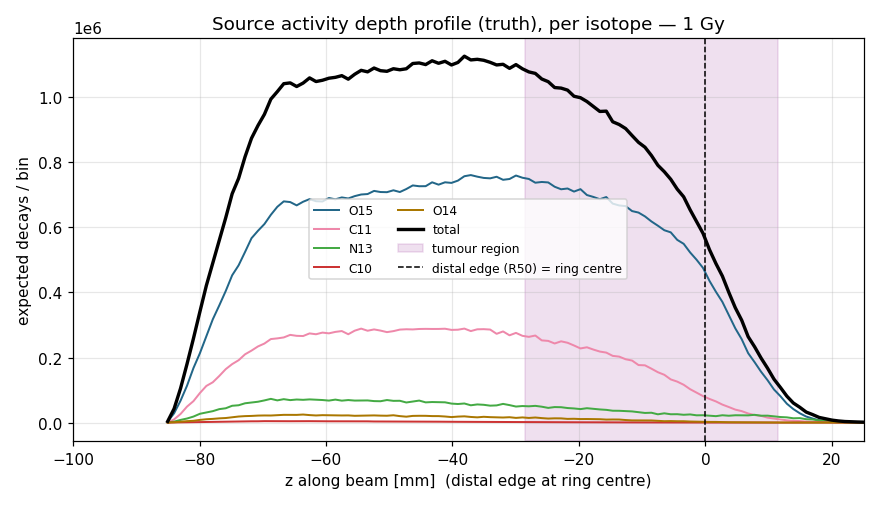
\includegraphics[width=0.86\textwidth]{figures/activity_truth.png}
\caption{Source activity depth profile (truth), per isotope, at 1\,Gy. \textbf{Tumour-centred}: the
SOBP dose-target centre is at $z=0$ (shaded band = target extent); the activity peaks proximal and
falls through its distal edge (R50, the range endpoint) ${\sim}+10$\,mm distal of the tumour. Source
level --- no scanner.}
\label{fig:activity}
\end{figure}

\subsection*{Timing: fixed acquisitions on the irradiation-end clock}

Time is measured from the \textbf{end of irradiation} (attr \texttt{t\_decay\_zero =
irradiation\_end}). Each product is a \textbf{fixed acquisition window} $[t_{\mathrm{del}},
t_{\mathrm{del}}+t_{\mathrm{ac}}]$: the patient arrives a delay $t_{\mathrm{del}}$ after the beam and
is imaged for a fixed $t_{\mathrm{ac}}=300$\,s (realistic in-room PET) --- \emph{not} a shrinking
window. The first round takes $t_{\mathrm{del}}\in\{120,180,300\}$\,s. Transport runs once over the
union window $[120,600]$\,s and each scenario is a band-cut of it ($t_{\mathrm{decay}}$ within the
window); on the irradiation-end clock the acquisition window, the physical decay, and the washout age
($=t_{\mathrm{decay}}$) factor cleanly, which is why this reframing removes the timing coupling that
made a shrinking-window start-cut error-prone.

Because the five isotopes span half-lives $19$--$1223$\,s ($^{10}$C $19$, $^{14}$O $71$,
$^{15}$O $122$, $^{13}$N $598$, $^{11}$C $1223$\,s), a later start loses the short-lived components
and reshapes the profile --- the timing rung of the range-degradation study.
Figure~\ref{fig:tstart} is the source truth for the three scenarios, each isotope scaled to its
expected decays in the window. From $t_{\mathrm{del}}=120$ to $300$\,s the total falls by
${\sim}2.3\times$ and the mix shifts from $^{15}$O-dominated toward the $^{11}$C tail; because those
isotopes sit at different depths, the distal edge reshapes. Every scanner sees this same source
evolution, modulated only by its axial acceptance.

\begin{figure}[htbp]
\centering
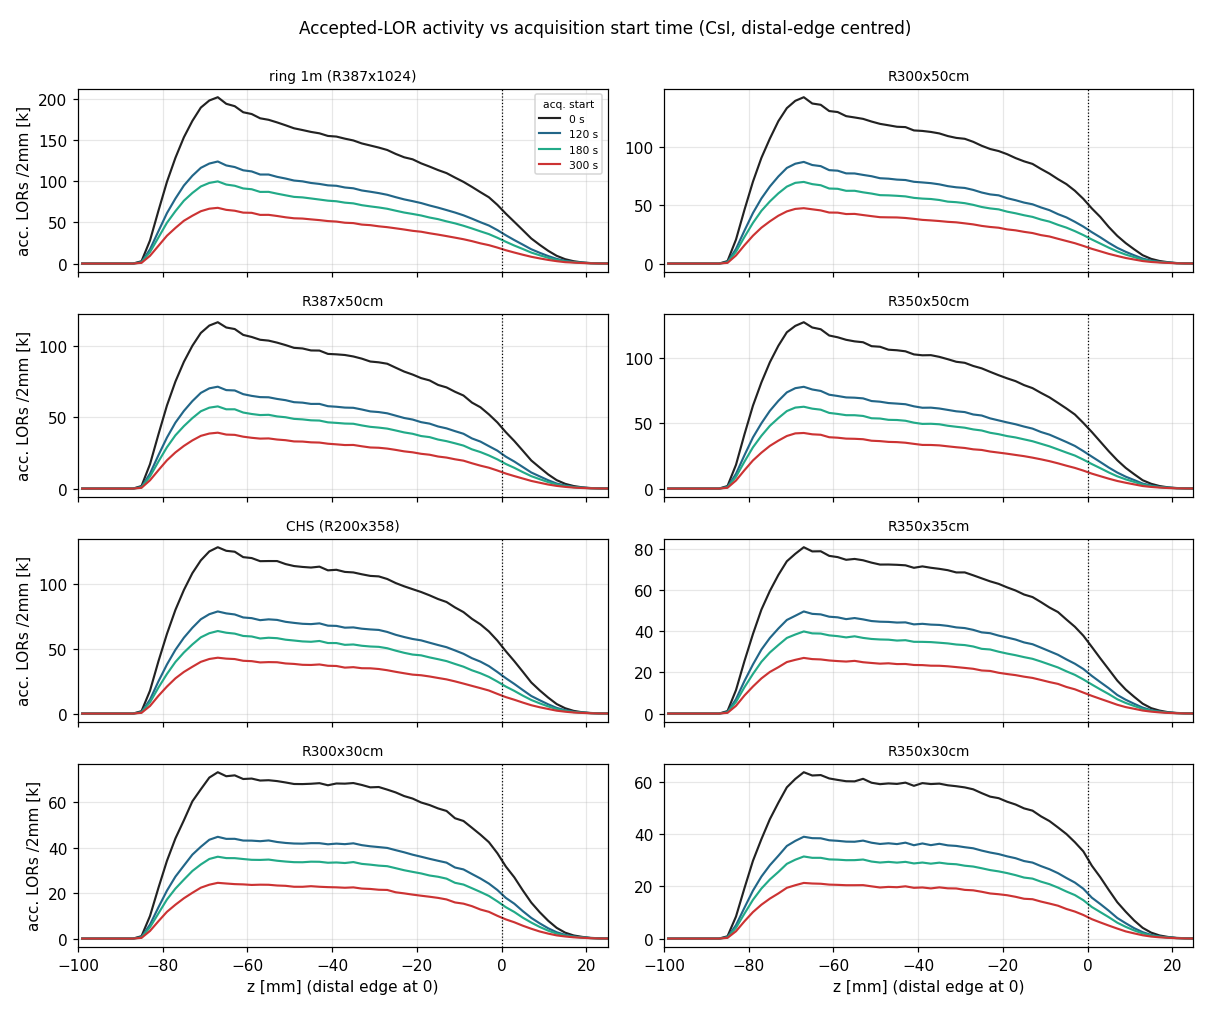
\includegraphics[width=\textwidth]{figures/activity_vs_tstart.png}
\caption{Source activity depth profile (truth), per isotope, for the three fixed acquisition
scenarios $t_{\mathrm{del}}=120/180/300$\,s (window $[t_{\mathrm{del}}, t_{\mathrm{del}}+300]$\,s) ---
each isotope scaled to its expected decays in the window. Delaying the start removes the short-lived
isotopes, cutting counts and reshaping the distal edge. Tumour at $z=0$; no scanner (source level).}
\label{fig:tstart}
\end{figure}

\subsection*{Isotope truth, and the first shard round}

Every LOR carries its emitting isotope (the \texttt{isotope} column), so the per-species content is
measured directly rather than inferred from a blind reconstruction. Figure~\ref{fig:shard} documents
the first v2 master round --- the reference detector \texttt{crysp\_ring\_1m\_csi\_2x0} (CsI), the
three scenarios, ten shards pooled each. The detected depth profile (left, trues) falls with delay
($26.8\to20.3\to12.2$\,M) and its distal edge --- the range endpoint --- reshapes; the isotope
composition (right) shows $^{15}$O depleting ($79\to62\%$) and $^{11}$C growing ($14\to29\%$) as the
start is delayed. The Mizuno brain washout survival $g_i$ is stamped per shard but \emph{not} applied
(left to \textsc{CryspBrainSim}); applied downstream it suppresses the long-lived $^{11}$C more than
the young $^{15}$O, partly opposing this drift.

\begin{figure}[htbp]
\centering
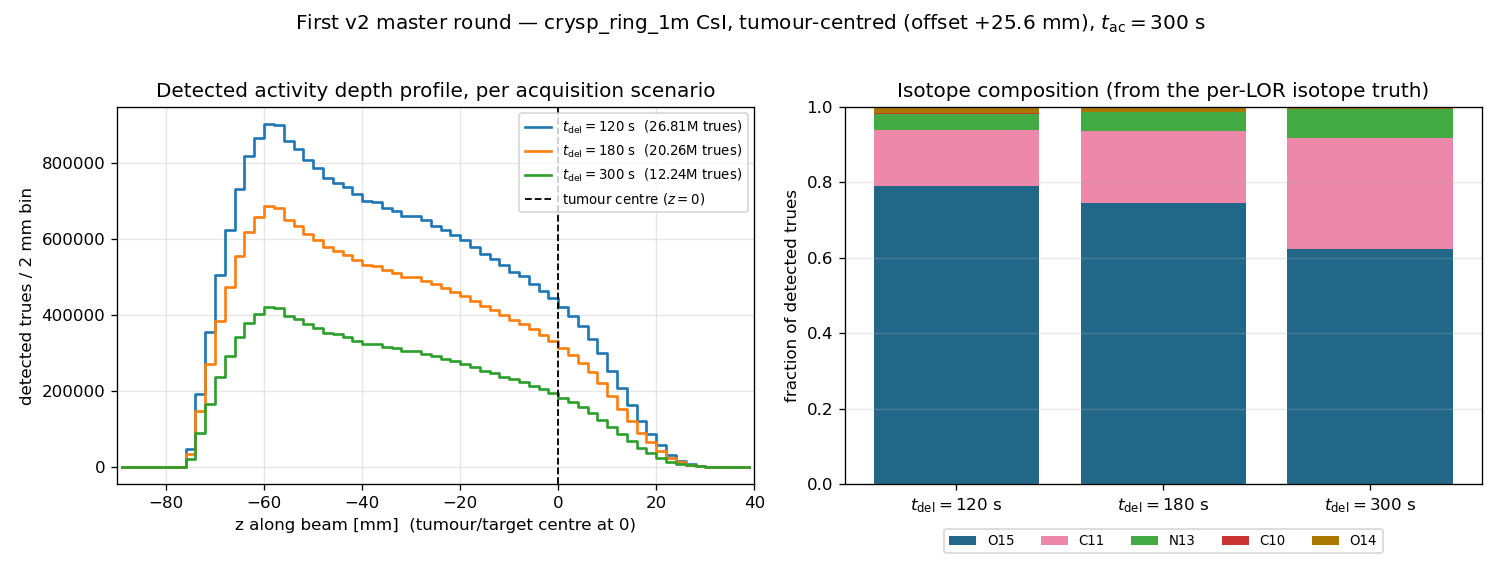
\includegraphics[width=\textwidth]{figures/shard_scenarios.png}
\caption{First v2 master round --- \texttt{crysp\_ring\_1m} CsI, tumour-centred, $t_{\rm ac}=300$\,s,
ten shards pooled per scenario. \textbf{Left:} detected activity depth profile (trues) vs the true
annihilation depth $z_0$, per acquisition scenario; counts fall and the distal edge reshapes as the
start is delayed (tumour at $z=0$). \textbf{Right:} isotope composition of the detected trues (from
the per-LOR isotope truth) --- $^{15}$O depletes and $^{11}$C grows with the delay.}
\label{fig:shard}
\end{figure}

\subsection*{The CsI three-ring survey}

Three CsI rings are produced in v2: the 1\,m flagship (\texttt{crysp\_ring\_1m}, $R\,38.7$\,cm /
AFOV $102$\,cm) and two compact head rings at $R\,35$\,cm (\texttt{crysp\_r35\_50cm} and
\texttt{crysp\_r35\_35cm}, AFOV $51$ and $36$\,cm), each across the three acquisition scenarios (ten
shards, $\Sigma M = 4.87\times10^{8}$ per leaf). Table~\ref{tab:csisurvey} and
Fig.~\ref{fig:csisurvey} summarise them. Acceptance grows with the axial FOV --- a larger solid angle
catches more gammas --- and falls with the arrival delay as the short-lived activity decays, from
$6.4\%$ (1\,m ring, $t_{\mathrm{del}}=120$\,s) down to $1.4\%$ ($36$\,cm ring, $t_{\mathrm{del}}=300$\,s).
Purity is geometry- and delay-independent at ${\sim}87\%$, dipping ${\sim}1$ point at the largest
ring (its larger solid angle admits marginally more phantom scatter). Whether the acceptance ordering
carries over to a $\sigma_R$ ordering is the downstream reconstruction question; these masters are
its clean, tumour-centred input.

\begin{table}[htbp]
\centering
\caption{CsI three-ring v2 survey (tumour-centred, $t_{\mathrm{ac}}=300$\,s): per acquisition
scenario, the selected-LOR yield (per shard; the master pools ten), the acceptance (selected LORs per
annihilation), and the purity (true fraction of the detected LORs).}
\label{tab:csisurvey}
\begin{tabular}{lccccc}
\hline
ring ($R$/AFOV) & $t_{\mathrm{del}}$ [s] & AFOV [cm] & LORs/shard & acceptance [\%] & purity [\%] \\
\hline
R38.7/102 & 120 & 102 & 3.09\,M & 6.35 & 86.7 \\
R38.7/102 & 180 & 102 & 2.34\,M & 4.80 & 86.7 \\
R38.7/102 & 300 & 102 & 1.41\,M & 2.90 & 86.7 \\
\hline
R35/51 & 120 & 51 & 2.09\,M & 4.29 & 87.4 \\
R35/51 & 180 & 51 & 1.58\,M & 3.24 & 87.4 \\
R35/51 & 300 & 51 & 0.95\,M & 1.95 & 87.4 \\
\hline
R35/36 & 120 & 36 & 1.47\,M & 3.01 & 87.6 \\
R35/36 & 180 & 36 & 1.11\,M & 2.27 & 87.7 \\
R35/36 & 300 & 36 & 0.67\,M & 1.37 & 87.7 \\
\hline
\end{tabular}
\end{table}

\begin{figure}[htbp]
\centering
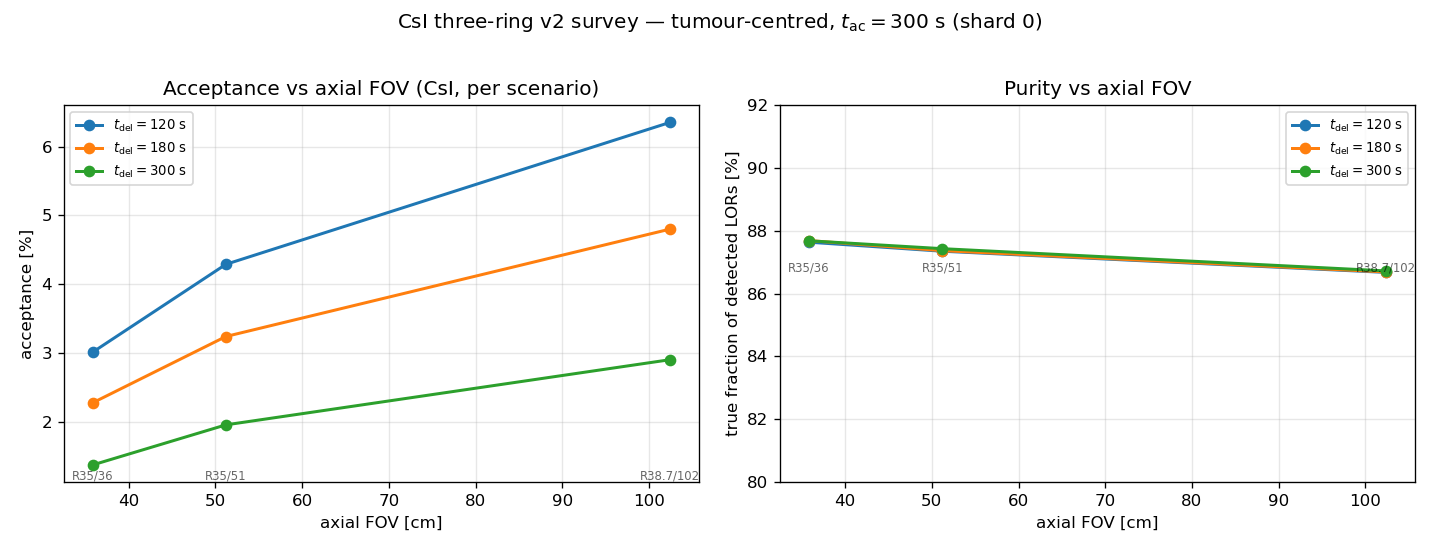
\includegraphics[width=\textwidth]{figures/csi_survey.png}
\caption{CsI three-ring v2 survey. \textbf{Left:} acceptance vs axial FOV, per acquisition scenario
--- it grows with the FOV (more solid angle) and falls with the arrival delay (short-lived activity
gone). \textbf{Right:} purity (true fraction of detected LORs) --- geometry- and delay-independent at
${\sim}87\%$, dipping slightly at the largest ring. Shard 0 (per-shard-stable quantities).}
\label{fig:csisurvey}
\end{figure}

\subsection*{The BGO arm, and CsI vs BGO}

BGO$_{195\mathrm{K}}$ is produced in v2 on the same three rings, but with the crystals 5\,cm further
out: BGO sits inside a cryostat, so $R(\mathrm{BGO}) = R(\mathrm{CsI}) + 5$\,cm --- giving
\texttt{crysp\_ring\_1m} ($R\,43.7$\,cm) and \texttt{crysp\_r40\_50cm}, \texttt{crysp\_r40\_35cm}
($R\,40$\,cm), at the \emph{same} axial FOVs (102/51/36\,cm) as their CsI counterparts.
Table~\ref{tab:bgosurvey} lists them; Fig.~\ref{fig:crystalcompare} compares the two crystals.

The trade is textbook. BGO's higher density stops far more gammas and, with its coarser $15\%$ energy
resolution, uses a lower photopeak cut ($413$ vs $472$\,keV) --- so its acceptance is ${\sim}2.4\times$
the CsI ($15.1\%$ vs $6.4\%$ at the 1\,m ring, $t_{\mathrm{del}}=120$\,s). But that same resolution
rejects scatter poorly, so BGO purity is ${\sim}73$--$77\%$ true against CsI's ${\sim}87\%$. Both
crystals order the same way with geometry (acceptance up with FOV, purity up toward the smaller
rings) and both are delay-independent in purity. Which crystal wins for range precision is the
downstream $\sigma_R$ question --- BGO offers more counts, CsI a cleaner sample; and the BGO count
advantage is already net of its $+5$\,cm cryostat radius.

\begin{table}[htbp]
\centering
\caption{BGO$_{195\mathrm{K}}$ three-ring v2 survey (tumour-centred, $t_{\mathrm{ac}}=300$\,s, crystals
at $R_{\mathrm{CsI}}+5$\,cm): per acquisition scenario, the selected-LOR yield (per shard; the master
pools ten), the acceptance, and the purity. Compare with the CsI Table~\ref{tab:csisurvey}.}
\label{tab:bgosurvey}
\begin{tabular}{lccccc}
\hline
ring ($R$/AFOV) & $t_{\mathrm{del}}$ [s] & AFOV [cm] & LORs/shard & acceptance [\%] & purity [\%] \\
\hline
R43.7/102 & 120 & 102 & 7.36\,M & 15.11 & 72.9 \\
R43.7/102 & 180 & 102 & 5.56\,M & 11.41 & 72.9 \\
R43.7/102 & 300 & 102 & 3.35\,M & 6.88 & 73.1 \\
\hline
R40/51 & 120 & 51 & 4.71\,M & 9.67 & 75.1 \\
R40/51 & 180 & 51 & 3.56\,M & 7.30 & 75.1 \\
R40/51 & 300 & 51 & 2.15\,M & 4.41 & 75.2 \\
\hline
R40/36 & 120 & 36 & 3.21\,M & 6.60 & 76.9 \\
R40/36 & 180 & 36 & 2.43\,M & 4.98 & 76.9 \\
R40/36 & 300 & 36 & 1.46\,M & 3.00 & 77.0 \\
\hline
\end{tabular}
\end{table}

\begin{figure}[htbp]
\centering
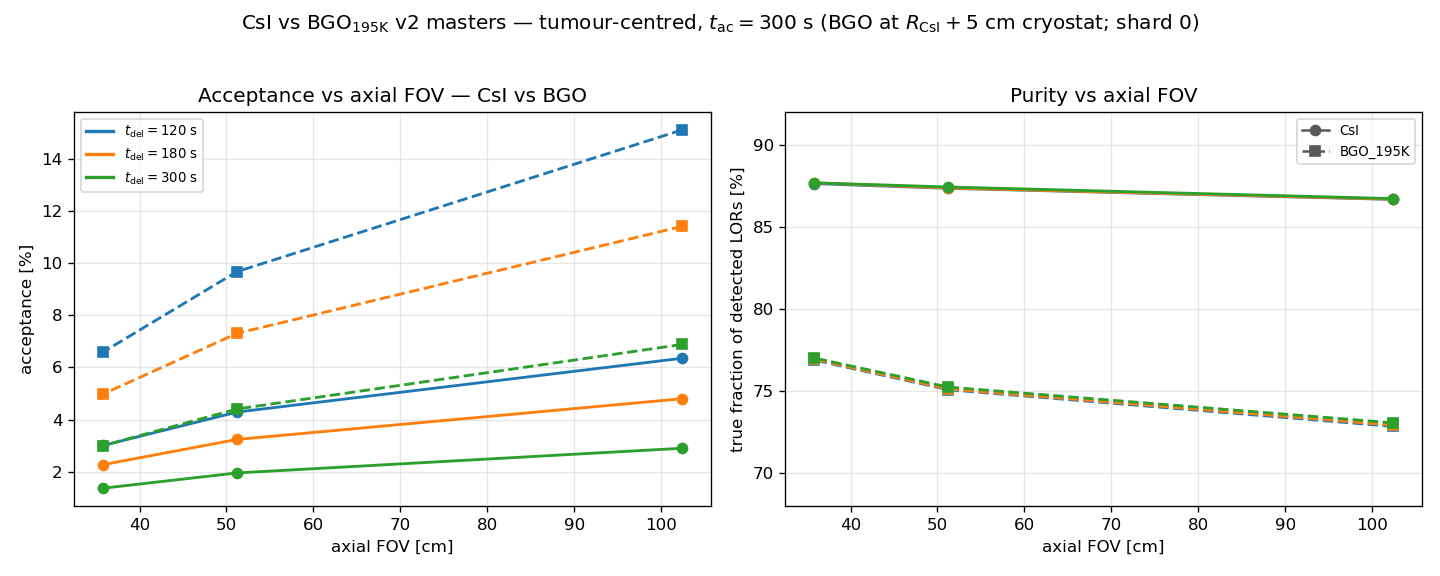
\includegraphics[width=\textwidth]{figures/crystal_compare.png}
\caption{CsI (solid, circles) vs BGO$_{195\mathrm{K}}$ (dashed, squares), v2 masters, per acquisition
scenario. \textbf{Left:} acceptance vs axial FOV --- BGO ${\sim}2.4\times$ the CsI (denser crystal,
lower photopeak cut), net of its $+5$\,cm cryostat radius. \textbf{Right:} purity --- CsI ${\sim}87\%$
vs BGO ${\sim}73$--$77\%$ (BGO's coarse resolution admits more scatter). Shard 0.}
\label{fig:crystalcompare}
\end{figure}

\section{Deferred refinements}
\label{sec:deferred}

Two refinements are scoped but deliberately deferred:
\begin{itemize}
\item \textbf{A standalone optical MC} of one monolithic block (PTFE-lined, SiPM plane on the
  instrumented face): a one-time computation per crystal system that would replace the
  ${\approx}1$ collection-efficiency assumption, quantify the DOI--time correlation
  (${\sim}0.13$--$0.15\ns$ systematic swing across the depth), and allow the readout floor to
  be split into its physical parts. Tracking the ${\sim}10^{12}$ optical photons of a
  production shard inline is not tractable, nor necessary: the parameterised result feeds
  eq.~\eqref{eq:stamp}.
\item \textbf{Scintillation rise time}: eq.~\eqref{eq:firstphoton} assumes the emission rate is
  maximal at $t=0$. A finite rise would degrade the first-photon term; at present it is
  absorbed into $\sigma_t$, pending cryogenic rise-time measurements.
\end{itemize}

\begin{thebibliography}{9}

\bibitem{Soleti2024}
S.~R.~Soleti, A.~Castillo, J.~Collar, M.~del Barrio-Torregrosa, C.~Echeverria, M.~Seemann,
D.~Zerzion and J.~J.~G\'omez Cadenas,
\emph{Cryogenic cesium iodide as a potential PET material},
JINST (2025), arXiv:2406.13598 [physics.ins-det].

\bibitem{Conti2009}
M.~Conti, L.~Eriksson, H.~Rothfuss and C.~L.~Melcher,
\emph{Comparison of fast scintillators with TOF PET potential},
IEEE Trans.\ Nucl.\ Sci.\ \textbf{56} (2009) 926.

\bibitem{Yamagishi2023}
S.~Yamagishi, K.~Miwa, S.~Kamitaki, K.~Anraku, S.~Sato, T.~Yamao et al.,
\emph{Performance characteristics of a new-generation digital bismuth germanium oxide PET/CT
system, Omni Legend 32, according to NEMA NU 2-2018 standards},
J.\ Nucl.\ Med.\ \textbf{64} (2023) 1990.

\bibitem{Janecek2012}
M.~Janecek,
\emph{Reflectivity spectra for commonly used reflectors},
IEEE Trans.\ Nucl.\ Sci.\ \textbf{59} (2012) 490.

\bibitem{Amsler2002}
C.~Amsler et al.,
\emph{Temperature dependence of pure CsI: scintillation light yield and decay time},
Nucl.\ Instrum.\ Meth.\ A \textbf{480} (2002) 494.

\end{thebibliography}

\end{document}
